\section{Sensorimotor Learning}
\label{sec:lb_sensorimotor}

Following the discussion above, the sensorimotor learning problem targets mapping raw sensor information to the actuator commands directly, for both manipulation and navigation tasks mainly through \textit{deep reinforcement learning}. A typical reinforcement learning pipeline is shown in Fig. \ref{fig:rlloop}

\begin{figure}[!ht]
   \centering
   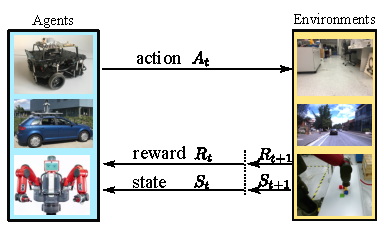
\includegraphics[width=0.65\columnwidth]{intro_figs/rlloop}
    \caption{The typical reinforcement learning loop for robotics tasks.
    The agent takes the action $\ba_{t}$ in state $\bs_{t}$, receives a reward $R_{t+1}$, and evolves to the next state $\bs_{t+1}$.}
   \label{fig:rlloop}
\end{figure}

In terms of manipulation, the tasks being considered for evaluating Deep Reinforcement Learning (DRL) algorithms are more standardized in the recent literature \cite{heess2017emergence,lillicrap2015continuous,mnih2016asynchronous,schulman2015trust,wu2017scalable}.
Most such works benchmark the proposed algorithms on standard tasks,
including \textit{reaching}, \textit{pushing}, \textit{pick-and-place}, etc.,
using the \textit{MuJoCo} simulator \cite{todorov2012mujoco}.
Below we focus on the works that are presented with real robotic experiments.

An asynchronous version of NAF is proposed in \cite{gu2016deep}.
Taking in the low dimensional states as inputs (joint angles, end-effector poses, as well as their time derivatives, and the pose of the target),
in addition to well-shaped reward signals, it allows the robot to learn a real-world door opening task in about $2.5$ hours in a completely end-to-end manner,
achieving a $100\%$ success rate.

Model-based approaches like guided policy search (GPS)\cite{levine2016end} can also successfully train deep visuomotor policies.
Their proposed visuomotor policy network takes as input monocular RGB images and passes them through several convolutional layers and a spatial soft argmax layer,
which are then concatenated with the robot configurations (joint angles, end-effector poses).
These representations are then passed through several fully connected layers and used to predict the corresponding motor torques.
Various experiments on a \textit{PR2} robot (with a $7$-DOF arm)
such as hanging a coat hanger on a clothes rack,
inserting a block into a shape sorting cube,
or screwing on a bottle cap have been demonstrated to validate the effectiveness of the approach.
This method, however, requires a known and fully observed state space,
which could limit its potential use cases.

Model-based DRL methods are also utilized by
\cite{finn2016deep} and \cite{tzeng2015towards},
learning useful state representations for generating successful control policies.
\cite{fu2016one} proposed one-shot learning of manipulation skills through model-based reinforcement learning by leveraging the neural network priors as a dynamic model.
Learning dexterous manipulation skills with multi-fingered hands,
for which model-based \cite{gupta2016learning, kumar2016optimal} and model-free \cite{popov2017data} DRL algorithms have been proposed and demonstrated in real robotic experiments,
is quite challenging.

While many works have carefully designed their reward structure to guide reinforcement learning,
some research \cite{martin2018learning} tried to speed up learning from only binary or sparse rewards,
under the observation that well-shaped rewards can often bias the learned control policy into potentially suboptimal directions.
In contrast, when only sparse reward signals are provided to the agent, the learner can discover novel and potentially preferable solutions.
To achieve this, alongside the policy learning for the main task, it learns policies (which they refer to as intentions) for a set of semantically grounded auxiliary tasks,
whose supervision signals can be easily obtained by the activation of certain sensors.
Then a scheduling policy is learned to sequence the intention-policies.
Their proposed algorithm is able to learn to solve challenging manipulation tasks from scratch,
such as stacking two blocks into a tower or cleaning up a desk by putting objects into a box with a lid that can be opened,
with a $9$-DOF robot arm. Moreover, in their real-world experiments, a single robot arm learns a lifting task in about $10$ hours.

Our work focuses on the robot navigation problem.
Autonomous navigation is one of the essential problems and challenges in mobile robotics.
It can roughly be described as the ability of a robot to plan and follow a trajectory through the environment to reach a certain goal location without colliding with any obstacles in between.
The recent literature has seen a growing number of methods proposed to tackle the task of autonomous navigation with DRL algorithms.
These works formulate the navigation problem as MDPs or POMDPs that first take in the sensor readings (colour/depth images, laser scans, etc.) as observations and stack or augment them into states,
and then search for the optimal policy that is capable of guiding the agent to navigate to goal locations in a timely and collision-free manner.
Below we discuss several representative works in this category that target the field of robotics.

Zhu \textit{et al.} \cite{zhu2017target} input both the first-person view and the image of the target object to the A3C model,
formulating a target-driven navigation problem based on the universal value function approximators \cite{schaul2015universal}.
The training of their model requires the output of the feature from a pre-trained \textit{ResNet}-$50$ \cite{he2016deep} and is performed in an indoor simulator \cite{kolve2017ai2}
where each new room is regarded as a new scene for which several scene-specific layers are added as another output head of the model.
The success rate for generalizing the navigation policies to new targets one step away from the trained targets is $70\%$,
and around $42\%$ for those that are two steps away.
For navigation tasks with optimal solutions of $17.6$ steps,
it achieves a $210.7$ average trajectory length after being trained on $100$ million frames with an A3C agent.
The trained policy was able to navigate a real robot inside an office environment after being fine-tuned on images collected from the real scene.

Zhang \textit{et al.} \cite{zhang2017deep} worked on a deep \textit{successor representation} formulation \cite{barreto2017successor, kulkarni2016deep} for the $Q$-value function,
targeting learning representations that are transferrable between related navigation tasks.
Following the observation that most of the \textit{value-based} DRL methods, such as DQN,
usually learn a black-box function approximator for the optimal value functions,
which makes how to transfer the knowledge gained from one task to a related task unclear,
they extended the \textit{successor feature representation} that decouples the learning of the optimal value functions into two parts,
learning task-specific reward functions, and learning task-specific features, and how those features evolve under the current task dynamics.
While this representation has been shown to work well on transferring learned policies to differently scaled reward functions and changed goals in fixed environments,
Zhang \textit{et al.} \cite{zhang2017deep} extended the formulation to cope with transferring policies to new environments.
